\chapter{Enhancing Spoken Language Translation with Prosody}
\label{chapter:transProse}
This chapter explores around the question of how can prosody be utilized in the framework of spoken language machine translation (SLMT). My motivation for this researched is enveloped around the applications automatic subtitling and dubbing in movie domain. The first goal of this chapter is to gain insights and prove that prosody is an essential element to consider in spoken language translation. This is performed through linguistic and corpus-based analysis on a bilingual expressive speech corpus (Section \ref{transProse:analysis}). Following, building of a neural machine translation system is explained in Section \ref{transProse:methodology}. This system serves both as a text translation baseline and a basis for incorporation of prosodic features in both input and output. Next, I perform experiments that utilize this system on movie-domain translation (speech-to-text and speech-to-speech). First, I explore the effect of prosodic punctuation restoration as a preliminary step to translation in Section \ref{transProse:Q1}. Secondly in Section \ref{transProse:Q2} I aim to improve text translation system through prosodically-enhanced input. And finally, for the aim of generating prosodic synthesis cues in a speech-to-speech translation pipeline, I report on the experiments building a translator that can handle prosodic input and output (Section \ref{transProse:Q3}). 

\section{Motivation and Background}
%introduction and problems faced
Spoken language machine translation is a type of machine translation (MT) where input and/or output to the system is spoken language. It is usually used in the context of translating from speech to text (through incorporation of ASR), or speech to speech (through incorporation of ASR and TTS). However, spoken language processing introduces its distinct challenges. For instance, in a system with speech input, the output of ASR lacks punctuation or phrase boundary information, which provides both linguistic and functional cues for translation. MT systems are usually trained with sentence or sentence-like phrases. However, ASR output can consist of partial sentences or long segments of tokens which in turn affects the functioning and quality of MT. Another issue arises in the case of a spoken input and output system. Prosodic information of the input speech is lost already in the first step. Thus, any communicative information residing in the input speech through prosody is not reflected in the translations and synthesized speech. 

%dubbing vs translation analogy
One can draw an analogy of the difference between spoken language translation and written language translation as the difference between book translation and movie dubbing. A book translator translates a book chapter by chapter, then paragraph by paragraph, and then sentence by sentence. All these segmentations are cued through the layout of the book, paragraph breaks and punctuation. Once at a certain sentence, the translator interprets the sentence in the original language of the book and then transforms it into the translation language following author's intentions. 

Although essentially a translation task, the art of dubbing a movie requires many more challenges. A similar segmentation process is followed but this time through scene information and actor turns. Once a line of an actor is transcripted, it can be segmented into sentences by looking both at grammatical and auditory aspects. The lines are then translated into the dubbing language by translators with the paralinguistic information such as the tone, intention and intensity noted. Finally, the voice actors vocalize the translated scripts respecting these paralinguistic aspects in the original version of the movie. 

%connecting analogy to the technological need
The additional tasks involved in the latter process should somehow be considered in an automatic translation/dubbing system of audiovisual content in order to obtain optimal results. The segmentation part requires tasks such as speech activity detection, speaker turn detection and ASR. The work in this chapter assumes that these tasks are already done perfectly and focuses on the translation part of the system and especially on the involvement of prosody to it. 

Specifically, I will address these three principal questions that involve prosody in the spoken language translation framework:

\begin{enumerate}
    \item How does prosodic punctuation restoration affect translation?
    \item Does pause encoding improve translation?
    \item Can pauses be translated jointly with lexical information?
\end{enumerate}

where the last one lying in the field of speech-to-speech translation. 

Before I embark on answering these questions, I will try to give the context to them with a linguistic and corpus study based on movie translation domain. This study is designed both to inspire the design of a prosodically enhanced translation model and also to help interpret experimental results. The questions will be answered with a practical methodology. 

The requirement posed by these questions is building of a prosodically enhanced translation model. Through this study, I aim to prove the need for inclusion of prosody in spoken machine translation pipelines and also to introduce a framework that would allow experimentation in this respect. 

As a remark, although there is previous work involving translation of TV-movie subtitles \citep{zora36755, zora8817}, this is to my knowledge the first work focusing on audio translation on movie domain. Spoken translation is even more interesting in this domain due to the highly expressive nature in movies. 

\section{Analyzing Significance of Prosody in Machine Translation}
\label{transProse:analysis}
In this section, I perform some example-based and statistical analysis on bilingual segments of the \textit{Heroes corpus}, which was presented in Chapter \ref{chapter:corpusWorks}. This corpus contains parallel English and Spanish speech segments from a dubbed TV series. The aim is to show how prosody is reflected in dubbing translation. Particularly, I focus on inter-lexical silent pauses as a prosodic feature. The first part demonstrates on a few examples in the corpus how pausing information influences translation, both for text and audio output. In the second part, I follow a statistical approach to prove significance of pausing in spoken translation. By pauses, I will always refer to silent pauses from this point as the dataset does not contain any information on filled pauses. 

\subsection{Example-based Analysis}
\label{subsection:heroes_examples}
In order to gain linguistic insights before building a data-driven model, selected parallel segments from the Heroes corpus are carefully inspected. Specifically, I investigate how does pausing as a prosodic feature reflects in the translation script. These are then compared to how a classic automated model performs with the same input sentence. All spoken samples presented throughout this chapter can be found in the thesis repository \footnote{\url{https://github.com/alpoktem/PhDThesis}}.

I will firstly examine the sample \textit{s2\_5\_0043} from the Heroes corpus. The original punctuated transcription of the English segment is: \textit{He pushed his way in, shoved a gun in my face. Next thing I know, he's flying through that glass.} Figure \ref{figure:heroes_viz_1} shows the Prosograph visualization of English and Spanish version of the sample. Yellow boxes, lines and circles below indicate unvoiced intervals between words, mean pitch and mean intensity, respectively.

%sample 1 - he pushed is way in. 
\begin{figure}[h!]
\begin{minipage}{\textwidth}
\begin{tabular}{c}
ENG \\
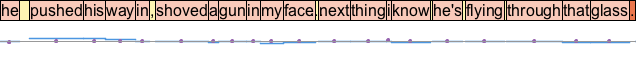
\includegraphics[height=1.2cm, width=\textwidth]{img/s2_5_0043-EN.png} \\
\end{tabular}
\end{minipage}
%\hfill
\begin{minipage}{\textwidth}
\begin{tabular}{c}
SPA \\
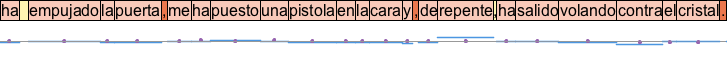
\includegraphics[width=\textwidth]{img/s2_5_0043-ES.png} \\
\end{tabular}
\end{minipage}
\caption{Segment pair s2\_5\_0043 from the Heroes corpus}
\label{figure:heroes_viz_1}
\end{figure}

Both segments are formed of 4 clauses. English segment consists of two sentences whereas in the Spanish segment these two sentences are joined with a linking word \textit{"y"} (and). Pauses are observed in all clause boundaries in English segment, whereas in the Spanish segment, a clause boundary pause is observed only after \textit{"de repente"} (\textit{lit.} suddenly, non-literal translation of \textit{"next thing I know"}). 

A fairly longer non-clause boundary pause is observed at the beginning of both sentences. 0.25 seconds of pause are observed after \textit{"he"} in English and 0.31 seconds of pause are observed after \textit{"ha"} (part of a compound verb to mark past tense) in Spanish. In the last clause in English, two short pauses are observed, which is not reflected in the Spanish sentence. However, when we listen to the Spanish segment, instead of a silent pause, a filled pause is observed where the word \textit{"ha"} is lengthened. 
With a focus on pauses, the following observations are made with respect to prosodic realizations in this particular segment pair. Firstly, silenced sections are not necessarily reflected in translation, even though they are induced by grammatical structures like clauses. Secondly, silences are sometimes reflected with respect to their position in the sentence and not from syntactic structure. This is partially due to the necessity that same sections need to be voiced in dubbing. And finally, it is seen that silent pauses can appear in a different form such as filled pauses. 

This parallel segment shows the complexity of the problem of prosodic transfer. It is hard to predict the prosodic realizations of the translation of a sentence only by looking at prosodic features in the input sentence. It is assumed that the English and Spanish versions of the segment are expressed in a similar fashion by the two actors, explaining these particular prosodic reflections. However, another voice actor could possibly dub this line in a different way with a different prosodic structure as well.  

%translation experiments
Next, a state of the art machine translation system is employed to see its performance in translating this example. Translations are performed using a state-of-the-art commercial MT system\footnote{Google Translate: \url{http://translate.google.com}}.  

\begin{description}
\item [Input sentence (ENG)] {\it He pushed his way in, shoved a gun in my face. Next thing I know, he's flying through that glass.}
\item [MT (ENG $\rightarrow$ SPA)] {\it Se abrió paso empujándome una pistola en la cara. Lo siguiente que sé es que está volando a través de ese cristal.}
\end{description}

What is noticed first is the mistranslations of some parts of the phrase. However, it is not our point to assess the quality of the translation in terms of correct word usage. The translated phrase represents the actions and objects in the source sentence well enough for our study. 

It is examined that the first two clauses in the English phrase are joined into one: \textit{Se abrió paso empujándome una pistola en la cara} (lit. \textit{He opened the way pushing a gun in my face}). Even though there is a comma separating the two clauses explicitly in the input sentence, this is not reflected in the translation. When we translate this section with punctuation marks removed we get a similar result:

\begin{description}
\item [Input sentence (ENG)] {\it he pushed his way in shoved a gun in my face} 
\item [MT (ENG $\rightarrow$ SPA)] {\it él se abrió paso empujándome una pistola en la cara}
\end{description}

The phrase, both prosodically and gramatically, is structured in a way that the speaker is explaining a sequence of actions: character pushing in and then pointing a gun on the speaker. Even though this is cued orthographically through punctuation, still the translation system is not able to capture this structure. An ideal translation that takes heed of the prosodic structure would be:

\begin{description}
\selectlanguage{spanish}
    \item \textit{Él se abrió paso, empujó una pistola en mi cara. Lo siguiente que sé, él está volando a través de ese cristal.}
\end{description}
\selectlanguage{english}

This example shows that a translation system that disregards the prosodic structure of the source sentence fails to translate in a way that was originally uttered. In a dubbing scenario, the presence of a pause in between two phrases should be reflected in the translation for two reasons: (1) to convey the same linguistic structure in translation and in turn (2) to ensure a synthesis reflecting the original phrasing. 

Next, I will list some examples where pausing is somewhat more directly transferred between original and dubbing language. Many samples of this type were found in the corpus. Three samples are demonstrated in Figures \ref{figure:heroes_viz_2} to \ref{figure:heroes_viz_4}. 

%this here's everything you had on you
\begin{figure}[h!]
\centering
\begin{tabular}{c}
ENG \\
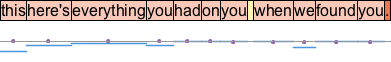
\includegraphics[height=1.2cm]{img/s2_5_0010-EN.png} \\
\end{tabular}
%\hfill
\\
\begin{tabular}{c}
SPA \\
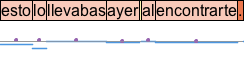
\includegraphics[height=1.2cm]{img/s2_5_0010-ES.png} \\
\end{tabular}
\caption{Segment pair s2\_5\_0010 from the Heroes corpus}
\label{figure:heroes_viz_2}
\end{figure}

\begin{figure}[h!]
\centering
\begin{tabular}{c}
ENG \\
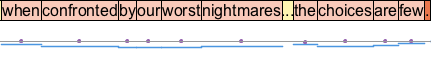
\includegraphics[height=1.2cm]{img/s2_5_0020-EN.png} \\
\end{tabular}
%\hfill
\\
\begin{tabular}{c}
SPA \\
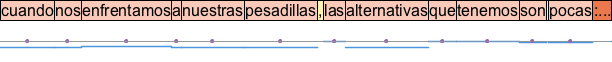
\includegraphics[height=1.2cm]{img/s2_5_0020-ES.png} \\
\end{tabular}
\caption{Segment pair s2\_5\_0020 from the Heroes corpus}
\label{figure:heroes_viz_3}
\end{figure}

\begin{figure}[h!]
\centering
\begin{tabular}{c}
ENG \\
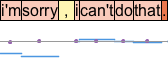
\includegraphics[height=1.2cm]{img/s2_5_0050-EN.png} \\
\end{tabular}
%\hfill
\\
\begin{tabular}{c}
SPA \\
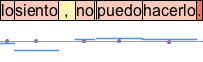
\includegraphics[height=1.2cm]{img/s2_5_0050-ES.png} \\
\end{tabular}
\caption{Segment pair s2\_5\_0050 from the Heroes corpus}
\label{figure:heroes_viz_4}
\end{figure}

Pause intervals can be directly traced at the phrase boundaries in both languages. This is, again, largely due to the necessity that voice-overs need to match the original voiced segments. What these translations suggest is that, a direct approach can be followed in transferring of pauses. Also, it is observed that paused slots are often marked with a punctuation in subtitles. 

In order to arrive to more concrete conclusions on the feasibility of a direct transfer of pauses and punctuation co-occurrence, a statistical study is conducted in the next subsection. 
 
\subsection{Corpus-driven Analysis}

Manual analyses done in the previous subsection are further extended to get a generalized behaviour of silent pauses in Heroes corpus. My motivation behind this study is to first, evaluate statistically how pausing is reflected in the dubbing translations in Heroes corpus, and second, how much pausing is related to punctuation in movie domain subtitles. 

\subsubsection{How is Pausing Reflected in Translations?}

A straightforward scheme is followed to evaluate how much of the silent pause events in English segments are reflected in the Spanish segments. To quantify this in the Heroes parallel corpus, first, number of segments with a pause event is counted for both English and Spanish segments. Then, number of segment pairs that contain a pause event only in English, only in Spanish and both in English and Spanish is calculated. A paused segment is defined as an unvoiced interval with a duration of minimum 0.05 seconds. See Table \ref{table:pausing} for the results. 

%pausing
\begin{table}[ht]
\centering
\begin{tabular}{lc}
\hline
\textbf{Event} & \textbf{\# Segments} \\ \hline
\textit{Pause in English segment} &  $3050$ \\
\textit{Pause in Spanish segment} & $3493$  \\
\textit{Pause in both English and Spanish} & $2539$  \\ 
\textit{Pause only in English segment} & $511$  \\
\textit{Pause only in Spanish segment} & $954$  \\ \hline
\end{tabular}
\caption{\label{table:pausing}Silent pause occurrences in English and Spanish segments of the Heroes corpus.}
\end{table}

It can be seen that in 83\% of the cases, a pause event in English segment is reflected in the Spanish segment. Other way around, in 72\% of the cases, a pause event in Spanish segment is reflected in the English segment. It can be deduced that pausing as a prosodic feature is reflected in the dubbing translations in majority of the cases. In this study, positions of the pauses are ignored. 

\subsubsection{To What Extend Pausing is Associated with Punctuation in Subtitle Transcripts?}

In the manual inspections performed in Subsection \ref{subsection:heroes_examples}, it was observed that many times pauses occur at punctuated slots between words in the subtitle transcription. Below, I explore this on a statistical basis in English and Spanish segments of the Heroes corpus similar to the study in TED talks presented in Section \ref{punkProse:analysis}. The importance of this study is to know how much pausing influence punctuation placement and vice versa in movie domain. Two directions of co-occurrence are observed: (1) how is a paused interval punctuated? and (2) to what extend punctuation infers a paused interval? I answer the first question in Figure \ref{figure:if_pause_then_punctuation} where distribution of punctuation events in paused intervals is shown. In English segments, among 1854 inter-word slots with a pausing, 80\% of them are annotated with a punctuation in the subtitle transcripts. The majority of the punctuation marks at these paused intervals are sentence ending punctuation marks (period [.], question mark [?], exclamation mark [!]), whereas comma [,] and ellipsis [...] consist of a smaller percentage. Spanish segments demonstrate a similar behaviour in terms of the ratio of punctuated slots with 78\% of them annotated with a punctuation mark. Whereas it is observed that commas tend to be paused more compared to English. These ratios indicate a higher punctuation probability of paused intervals compared to the conference talk transcripts. 

\begin{figure}[h]
    \centering
    \begin{minipage}{.5\textwidth}
        \centering
        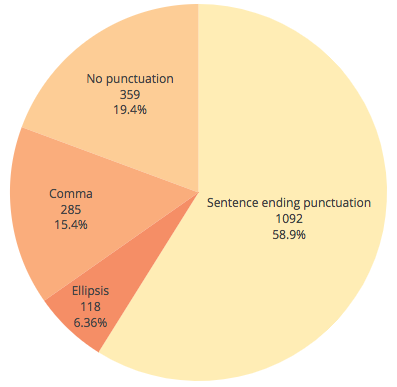
\includegraphics[width=\linewidth]{img/if_pause_then_punctuation_ENG.png}
    \end{minipage}%
    \begin{minipage}{0.5\textwidth}
        \centering
        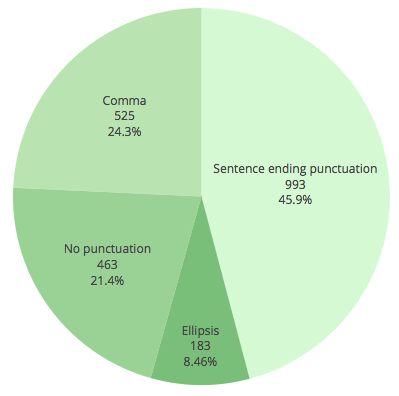
\includegraphics[width=\linewidth]{img/if_pause_then_punctuation_SPA.png}
    \end{minipage}
    \begin{minipage}{.5\textwidth}
        \centering
        English
    \end{minipage}%
    \begin{minipage}{0.5\textwidth}
        \centering
        Spanish
    \end{minipage}
\caption{Punctuation distribution at paused ($ > 0.05$ s) intervals in English segments(1936 in total) of the Heroes corpus.}
\label{figure:if_pause_then_punctuation}
\end{figure}

Secondly, Table \ref{table:if_punctuation_then_pause} shows the distribution of pausing events at inter-lexical intervals where a punctuation occurs. Looking at English segments, when all punctuation marks are considered, there is a pause in that interval with a 58\% of probability. However, when only sentence ending punctuation marks are considered this percentage rises to 75\%. It can be deduced that a sentence boundary is a highly discriminating cue for a pausing event between two words. However, the ratio of pause presence at occurrences of comma is quite low (39\%). Whereas in Spanish segments, commas seem to be paused much more with a 60\% of them marking a short pause of 420 ms in average. Punctuation marks that act as a sentence boundary also mark a pause more than in English segments (86\%). Both these contribute to a higher distribution of pausing at punctuation points. 72\% of punctuation marks are paused, which is 14\% higher than in English segments. 

Through these studies it can be confirmed that pausing is a highly correlated phenomena with punctuation in movie domain. Comparing to the transcriptions of TED talks, the numbers indicate a higher percentage of punctuation-pause correlation in movie subtitles. 

Two insights that could be taken from these results regarding movie domain machine translation is that: (1) Punctuation restoration can benefit more from the use of prosodic features such as pauses and (2) prosodic features can complement punctuation in acting as cues for machine translation. 

%if_punctuation_then_pause table
\begin{table}[ht]
\centering
\begin{tabular}{>{\centering\arraybackslash} m{0.25\linewidth} >{\centering\arraybackslash} m{0.16\linewidth} >{\centering\arraybackslash} m{0.16\linewidth} >{\centering\arraybackslash} m{0.14\linewidth} >{\centering\arraybackslash} m{0.16\linewidth}}
\textbf{Punctuation event} & \textbf{\#Occurrences} & \textbf{\#Occurrences w/ pause} & \textbf{Percentage of paused} & \textbf{Mean pause duration (s)}\\ \hline
\textbf{English} & & & & \\
 \hline
\textit{Punctuated interval}      &  $5\,429$ & $3\,152$ & $58\%$ & $0.81$ \\
\textit{Sentence boundary}        &  $2\,549$  & $1\,913$ & $75\%$ & $1.02$ \\
\textit{Comma}                    &  $2\,652$ & $1\,038$ & $39\%$ & $0.38$  \\ 
\textit{Ellipsis}                 &  $228$ & $201$ & $88\%$ & $0.94$ \\ \hline
\textbf{Spanish} & & & & \\
 \hline
\textit{Punctuated interval}      &  $4\,935$ & $3\,580$ & $72\%$ & $0.77$\\
\textit{Sentence boundary}        &  $1\,856$  & $1\,606$ & $86\%$ & $1.11$\\
\textit{Comma}                    &  $2\,718$ & $1\,653$ & $60\%$ & $0.42$  \\ 
\textit{Ellipsis}                 &  $361$ & $321$ & $88\%$ & $0.83$ \\ \hline
\end{tabular}
\caption{\label{table:if_punctuation_then_pause}Pause presence in punctuated intervals in English and Spanish segments of Heroes corpus.}
\end{table}

\section{Methodology}
\label{transProse:methodology}

Having the intuition gained from examining prosodic parallelisms in the bilingual segments of the Heroes corpus, I embark on building a system that can learn and generate prosodic structures in a neural machine translation setup. This section explains the MT framework built in order to carry out experiments to answer the questions we listed earlier. Before diving in the technical specifications of the system built, I will list the requirements defined prior to the implementations:

\begin{enumerate}
    \item Translation will be in movie domain. This is mainly because of our motivation for gaining insights for the automatic subtitling and dubbing use cases. 
    \item System will be extended incrementally i.e.~we will start from a basic text translation system and then add on it first prosodic input and then prosodic output. 
    \item Prosodic encoding and decoding will be built within the translation system; i.e.,~text and prosodic encoding and decoding parameters will be learned jointly. 
    \item The system should be able to compensate for the scarcity of spoken parallel data. 
\end{enumerate}

In order to address these requirements, a system is built that can learn translation of textual and prosodic features jointly. I will refer to this system as \textit{TransProse} for simplicity. Design and subtleties of this model are explained in the next subsection \ref{transProse:methodology:model}. Next, data sources that suit best for our problem has to be selected. Collected and acquired corpora and our preprocessing steps are detailed in subsection \ref{transProse:methodology:data}. 

\subsection{Neural Translation Model}
\label{transProse:methodology:model}

%Sequence-to-sequence modeling has proved in recent years that it is one of the most advanced models for modelling automatic translation \cite{sutskever}. This model works by \textit{encoding} a phrase in the source language to a single vector and then \textit{decoding} it into the phrase in the target language. A drawback of this classic encoder-decoder architecture is that the entire encoded sequence has to go through one vector acting as a funnel to be decoded into target sequence. This problem was addressed by the introduction of attention mechanism \citep{bahdanau, luong}, which lets the decoded sequence to focus on relevant areas of the encoded sequence.

TransProse framework is based on a sequence-to-sequence network with attention mechanism, which was explained earlier in Chapter \ref{chapter:sota}. For that reason, I will not go deep into the core of the architecture but I will explain more how it was extended to handle prosodic input and output. 

\subsubsection{Encoding Text Tokens and Prosody}

\begin{figure}
\centering
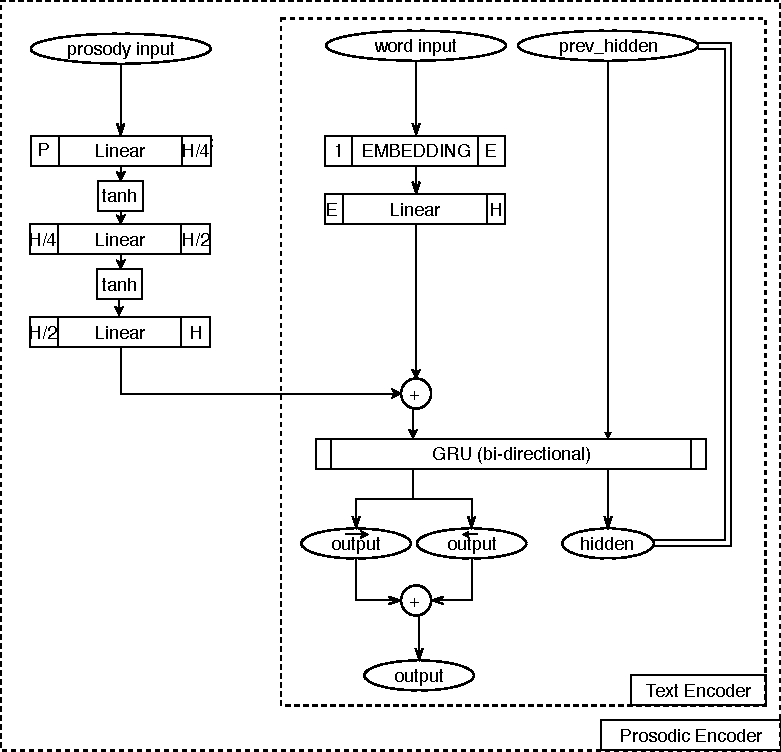
\includegraphics[width=0.7\linewidth]{img/TransProse_Encoder.pdf}
\caption{TransProse sequence-to-sequence translation encoder with prosodic input.}
\label{figure:transprose_encoder}
\end{figure}

The encoder of the system is illustrated in Figure \ref{figure:transprose_encoder}. The text encoder part (inner box) takes word token indexes as input and passes them through an embedding layer then a linear layer to obtain word vectors of size $H$. Then, this vector is passed to a bidirectional GRU layer, outputting hidden and an output vectors in both directions at each step. The forward and backward output vectors are then summed in order to obtain an output of size $H$ for each input token. 

Encoding jointly with the added prosodic features is depicted in the outer box of the same figure. Note that prosody input vector carries any number of prosodic/acoustic features that belong to the word token at that timestep. This number is denoted with $P$. A separate encoding sequence is followed by the prosodic features. The input features are converted to a vector of size $H$ in a gradual fashion where a linear layer is followed by a non-linearity at each step. Once it is the same size of the GRU input layer, it is summed with the encoded word input and introduced to the bidirectional layer together with the input word token representation. Output vectors at each timestep are then passed on through the decoder. 

\subsubsection{Decoding Text Tokens and Prosody}

\begin{figure}
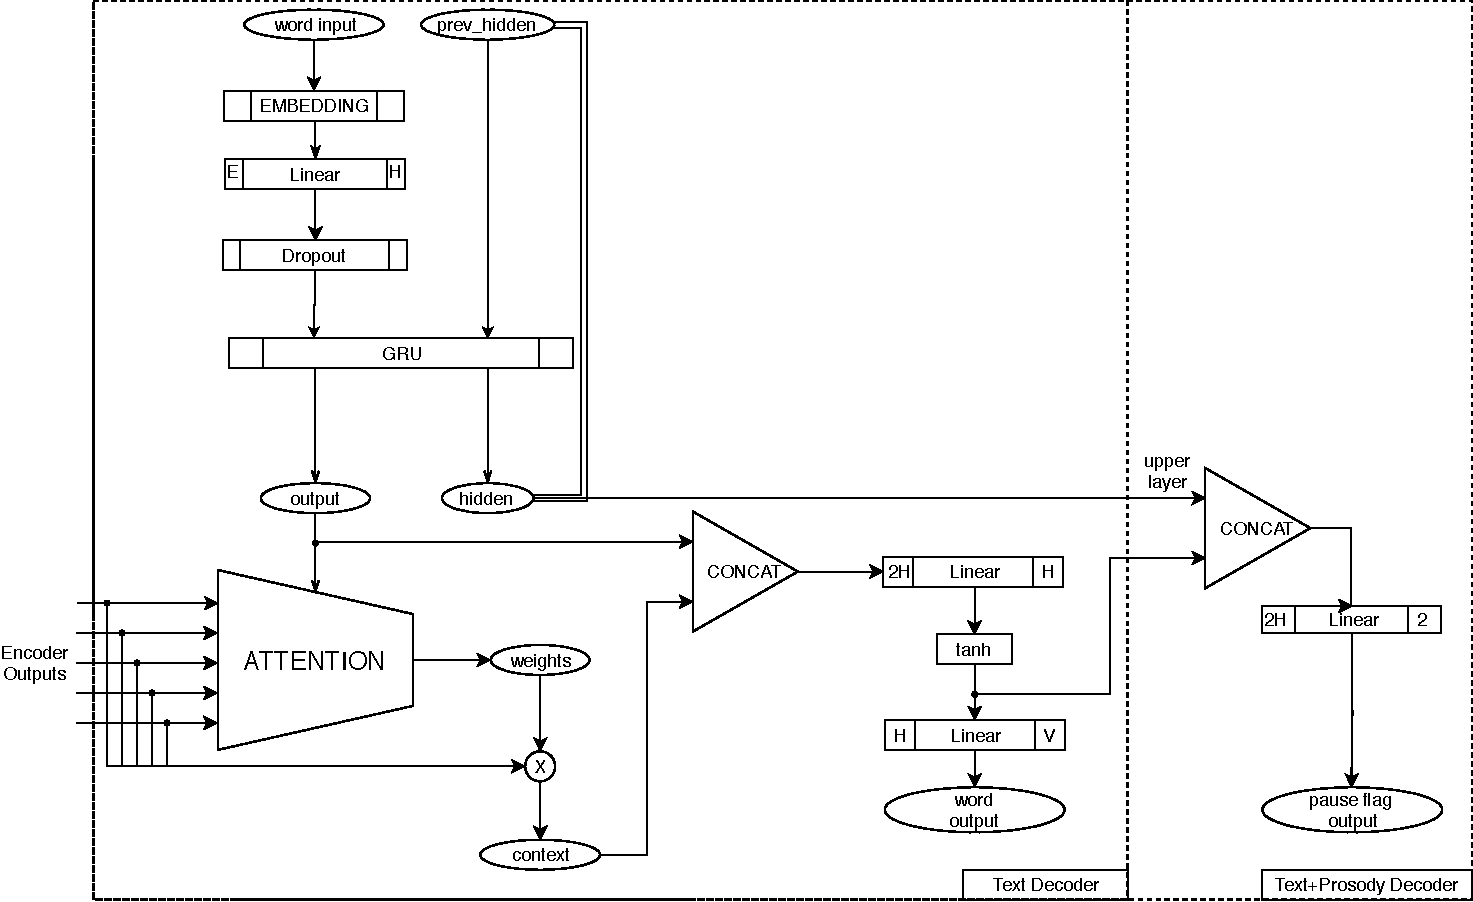
\includegraphics[width=\linewidth]{img/TransProse_Decoder.pdf}
\caption{TransProse sequence-to-sequence translation decoder with prosodic output.}
\label{figure:transprose_decoder}
\end{figure}

As illustrated in Figure \ref{figure:transprose_decoder}, the decoder is also designed to output either text tokens only or accompanied with their corresponding prosodic features. During training, target sequence tokens are input and passed through first, the embedding layer, then a linear layer followed by a dropout layer until it reaches the GRU layer. The output of the GRU layer is used to determine the attention weights according to each of the effect of the encoder output effect on that particular target token. The attention model is based on the global attention model in \cite{luong}. The weights vector for output at timestep $t$ is calculated as in Equation \ref{equation:attn1}, where $h _ { t }$ stands for GRU output in decoder side and $h _ { s }$ on the target side. General scoring function is used as the scoring function ($\operatorname { score } \left( h _ { t } , \overline { h } _ { s } \right) = h _ { t } ^ { \top } \mathbf { W } _ { a } \overline { h } _ { s }$). A general overview of the implementation of the neural attention architecture is illustrated in Figure \ref{figure:transprose_attn}.

\begin{equation}
\label{equation:attn1}
a _ { t } ( s ) = \operatorname { align } \left( h _ { t } , \overline { h } _ { s } \right) = \frac { \exp \left( h _ { t } ^ { \top } \mathbf { W } _ { a } \overline { h } _ { s } \right) } { \sum _ { s } \exp \left( h _ { t } ^ { \top } \mathbf { W } _ { a } \overline { h } _ { s } \right) }
\end{equation}
 

% \begin{equation}
% \label{equation:attn2}
% \operatorname { score } \left( h _ { t } , \overline { h } _ { s } \right) = h _ { t } ^ { \top } \mathbf { W } _ { a } \overline { h } _ { s }
% \end{equation}

\begin{figure}
\centering
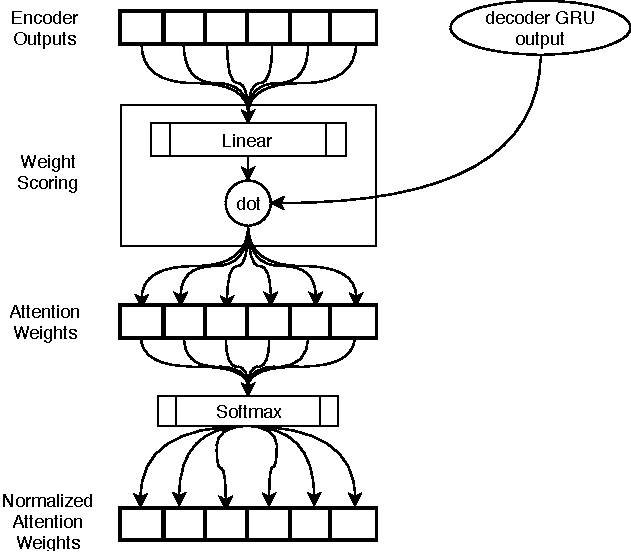
\includegraphics[width=0.7\linewidth]{img/TransProse_attn.pdf}
\caption{Attention mechanism in the TransProse decoder.}
\label{figure:transprose_attn}
\end{figure}

After the attention weights are calculated, encoder outputs are multiplied with these weights and averaged to obtain the context vector. Context vector is then concatenated with the decoder output and eventually used to calculate the vocabulary sized one-hot word token output. 

The depiction of the decoder illustrated in Figure \ref{figure:transprose_decoder} has one type of prosodic outputs: pause flag.
Flag outputs are of size 2 and are designed to fire when a pause is predicted after the current predicted word of the timestep. 

Both in encoder and decoder, word embedding layer is initialized with pre-trained word vectors, and is updated during training. 

\subsubsection{Learning Procedure}
%Two stage training and parameter loading
A translation model enhanced with prosodic input and/or output is obtained in two stages. First, training is performed on parallel text data updating only the parameters belonging to the text encoder and decoder. On a second stage, training is performed on prosodically annotated parallel data with the joint text+prosody encoder/decoder components. Before starting the second stage training, the extended text+prosodic architecture is initialized with the pre-trained first stage parameters. While training on prosodic data, all parameters are updated, where prosodic model components are trained from scratch. 

%Objective functions
In order to calculate gradients for the model to converge while training, loss functions has to be defined for the model outputs. The loss function compares the prediction of the model to the gold output and back-propagates to decide how the model parameters should be updated. For text token and flag-based outputs, masked cross entropy is used. Average loss is calculated after each batch by summing each individual loss with its respective weight, as in Equation \ref{equation:loss}:

\begin{equation}
    \label{equation:loss}
    { L }_{ total }= { \lambda }_{ word }\cdot { L }_{ word }+ { \lambda }_{ pauseflag }\cdot { L }_{ pauseflag }
\end{equation}

In text training, total loss function is only the loss coming from word token predictions. In audio training, loss weights ${ \lambda }_{ word }$ and ${ \lambda }_{ pauseflag }$ are set to $1.0$ and $10.0$ respectively. In this work, pause flag output is employed only in the experiment reported in Section \ref{transProse:Q3}. 

For parameter optimization, Adam \citep{DBLP:journals/corr/KingmaB14} is used. After each training epoch, model is validated on a smaller validation set. Training is continued until no improvement is noted in terms of total loss in the validation set in the last three epochs. 

\subsection{Data and Data Preprocessing}
\label{transProse:methodology:data}

Training is performed in two stages with two types of data, a parallel text corpus and a prosodically annotated parallel spoken audio corpus. \textit{OpenSubtitles corpus} and \textit{Heroes corpus} were used respectively for the two stages of the task. 

\subsubsection{Parallel Text Dataset}
In order to keep consistent in the movie domain, text data are also obtained from movie based resources. \textit{OpenSubtitles} collection\footnote{\url{http://www.opensubtitles.org/}} provides parallel text obtained from movie and series subtitles and is provided freely in the \textit{OPUS website} \citep{Lison2016OpenSubtitles2016EL}. The \textit{OpenSubtitles2018} release\footnote{\url{http://opus.nlpl.eu/OpenSubtitles2018.php}} contains 1,782 bilingual text pairs among 62 languages. For the English-Spanish pair more than 61 million sentence pairs are available. 

The text dataset to train TransProse models is gathered from this set. The dataset size was restricted to 5 million sentence pairs to accommodate training in reasonable amount of time. Sentence pairs for this set of 5 million sentence pairs, which we call the \textit{opus5mm} set, is obtained by a simple set of filters selecting from the original corpus. These filters are: 

\begin{enumerate}
    \item Sentences shouldn't contain more than a certain number of tokens (40 in this case),
    \item Sentences shouldn't contain any non-alphanumeric characters,
    \item Sentence should only consist of tokens in a pre-determined vocabulary of most frequent 30,000 tokens in the whole corpus.
\end{enumerate}

These filters were determined in order to ensure a training set as clean as possible. Since the corpus is derived automatically from subtitles registered in \textit{opensubtitles.org}, it is likely to come across badly written sentences or misalignments. Also, subtitle segments where auditory or visual annotations are made was filtered out. These subtitle segments contain information on speaker, background music, voice characteristics and even signatures of the subtitle authors and are marked with usage of XML-style tags or other non-alphanumeric characters. 

Another important characteristic of the movie subtitles is that translations are not necessarily literal. The differences are caused by the nature of subtitling, e.g. sentences are cut short to fit on the screen or some spoken remarks are omitted to simplify reading. This feature makes movie subtitles sub-optimal for training translation models. 

The \textit{opus5mm} dataset consists of 5 million sentence pairs plus 10,000 pairs for validation and 10,000 for testing purposes. For tokenization, \textit{NLTK tokenizer} \citep{nltk} is used with a modification on English enclitics. Words tokens were separated from apostrophes. For example the word ``I'll'' consists of two tokens: ``I'' and ``'ll''. 

\subsubsection{Parallel Speech Dataset}
For the second stage training involving prosodic parameters, \textit{Heroes corpus} is used. The experiments described in this chapter are performed on a pre-release version of the corpus that consisted of 7225 parallel segments. Two training-test-validation partitionings generated from this dataset are described in Table \ref{table:heroes_partitions}. The first partitioning \textit{heroes-v1} is generated by taking 80\% of the shuffled segment pairs as training set and dividing the rest into two to be used as test and validation sets. The second partitioning \textit{heroes-v2} is generated in a more manual fashion. First, 138 segment pairs were manually picked from \textit{heroes-v1} test set, that ensured a translation well enough to be used in the prosodic prediction experiments. Secondly, after shuffling the rest of the segment pairs, 200 were chosen randomly for the validation set and the remaining 6887 segments were allocated as training set. 
\begin{table}[ht]
\centering
\begin{tabular}{>{\centering\arraybackslash} m{0.15\linewidth} >{\centering\arraybackslash} m{0.15\linewidth} >{\centering\arraybackslash} m{0.15\linewidth}  >{\centering\arraybackslash} m{0.15\linewidth} }
\hline
\textbf{Dataset} & \textbf{\#Training samples} & \textbf{\#Validation samples} & \textbf{\#Testing samples} \\ \hline
\textit{heroes-v1} & 6141 & 542 & 541 \\
\textit{heroes-v2} & 6887 & 200 & 138\\\hline
\end{tabular}
\caption{\label{table:heroes_partitions} Heroes corpus partitioning versions and number of train, validation and testing set samples. }
\end{table}

\subsubsection{Punctuation Handling and Prosodic Sequence Representation}
%oui
% In the neural machine translation model described above, prosodic features are assumed to be parallel to the tokens that form the input and output sequences. That is, each token has its prosodic features associated to it. This goes parallel with the how the movie segment data is stored in the speech corpus used. In \textit{Heroes corpus}, prosodic features are calculated and stored for every word. These features include pause coming after that word (\textit{pause after}, \textit{mean F0} and \textit{mean intensity}) associated with that word. Punctuation marks are also features of the words. Two punctuation features are associated with each word: \textit{punctuation before} and \textit{punctuation after}. These structures needed to be taken into account during the design of the translation pipeline. 

In the neural machine translation model described above, prosodic features are assumed to be parallel to the tokens (words and punctuation) that form the input and output sequences. Resulting from this design choice, punctuation tokens also need to carry prosodic features. Although this is logically unintuitive, it was the approximation that was made. Figure \ref{transprose:figure:q3:assequence} shows an example of an utterance from the speech corpus and its representation as an input sequence to the neural network. The original segment consists of 4 tokens as can be seen in the \textit{Prosograph} illustration. After tokenization, the input sequence results ends up with 7 tokens (including the END token). F0 and intensity features are copied into the punctuation mark tokens attached to a word.

\begin{figure}[h!]
\centering
\begin{minipage}[t]{0.37\textwidth}
\begin{tabular}{c}
Speech segment \\
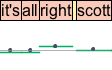
\includegraphics[height=1.8cm]{img/s3_12_0124.png} \\
\end{tabular}
\end{minipage}
%\hfill
\\
\begin{minipage}[t]{\textwidth}
\begin{tabular}{c}
Sequence representation \\
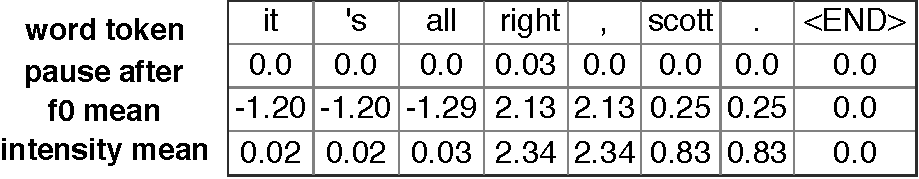
\includegraphics[height=2.3cm]{img/s3_12_0124_assequence.pdf} \\
\end{tabular}
\end{minipage}
\caption{Segment \textit{s3\_12\_0124\_EN} from the Heroes corpus and its sequence representation.}
\label{transprose:figure:q3:assequence}%lalala
\end{figure}

%\mireia{didn't you use the 0.01 and 0.99 percentiles for minimum and maximum values?}
F0 and intensity features, which were already normalized with respect to the speaker norm, are further normalized within $-1$ to $+1$ representing corpus minimum and maximum. Pause duration was normalized within $0$ and $1$, 1 meaning a pause duration of 10 seconds. 

\subsubsection{Further Implementation Details}
The architecture described in this section is implemented with PyTorch\footnote{\url{https://pytorch.org/}}. Text models were trained on graphical processing units (GPU)\footnote{GPU was kindly donated by NVIDIA through the GPU grant program} and second stage prosodic models were trained on CPU. Other hyperparameters used while training are listed in Table \ref{table:transprose_hyperparameters}.

\begin{table}[ht]
\centering
\begin{tabular}{>{\centering\arraybackslash} m{0.39\linewidth} >{\centering\arraybackslash} m{0.1\linewidth} }
\hline
\textbf{Hyperparameter} & \textbf{Value} \\ \toprule
\textit{Encoder learning rate} &  0.0001 \\
\textit{Decoder learning rate} & 0.0005 \\
\textit{Batch size} & 64  \\ 
\textit{Hidden layer size} & 512  \\
\textit{Number of GRU hidden layers} & 2  \\
\textit{Decoder dropout rate} & 0.1  \\
\textit{Gradient norm clip rate} & 50.0  \\
\textit{Word vocabulary size (EN-ES)} & 30,000  \\
\textit{Maximum sequence size} & 40  \\\bottomrule
\end{tabular}
\caption{\label{table:transprose_hyperparameters}Hyperparameters used in the experiments with TransProse architecture. }
\end{table}

Initial word vectors were trained using the \textit{gensim} library \citep{gensim}. These vectors were trained from English and Spanish segments in the complete OpenSubtitles corpus. An optimal vocabulary was created with a combination of the most frequent 30,000 tokens from this corpus with the tokens in the Heroes corpus. 

\section{Experiments}
\label{transpros:experiments}

In this section I will explain the following three stages of experimentation that is based on the proposed TransProse framework:

\begin{enumerate}
    \item How does prosodic punctuation restoration affect translation?
    \item Does pause encoding improve translation?
    \item Can pauses be translated jointly with lexical information?
\end{enumerate}

\subsection{How Does Prosodic Punctuation Restoration Affect Translation?}
\label{transProse:Q1}

In previous chapter, it was stated that punctuation restoration of transcriptions has an important role for subsequent processing steps such as machine translation. This section focuses on this very statement and explores the effect of punctuation restoration in transcripts on translation. Principal functionality of punctuation in a machine translation system is that it segments source input into meaningful units through sentence structure, which in turn gives cues on the output structure. Most state-of-the-art translation systems take sentences as units to translate. The type of punctuation that ends the sentence signifies if it is a statement, interrogation or exclamation. This does not only affect what punctuation mark should be placed at the end of the target sentence but also the translation itself. Moreover, intra-sentence segmentations through usage of commas signal which types of word groupings (e.g.~clauses) should be carried to the target translation.

The first question that this section explores is: To what extend source input punctuation affects machine translation performance? Secondly, assuming to have unpunctuated transcriptions of an audiovisual content, e.g.~coming from ASR, how can we recover from this loss with punctuation restoration as a preliminary process step to machine translation? Thirdly and mainly, the effect of using prosody and domain-adapted punctuation and translation models is explored. 

\subsubsection{Experimental Setup}

The experiments are based on the movie domain focusing on the use case of translation of TV series. Translation models were trained on \textit{opus5mm} set and then adapted to the \textit{heroes-v1} set. 

In order to quantify the difference in performance caused by punctuation, the source sentences are sent to translation with and without the punctuation marks already present in the dataset. These marks are the annotated punctuation in the original English subtitles of the TV series. %Segments with the original punctuation are called \textit{subtitle punctuation}.  and \textit{no punctuation} with punctuation marks removed. 

Punctuation restorations are performed over English segments with models obtained using the \textit{punkProse} framework presented in Chapter \ref{chapter:punkProse}. Four models that were trained specifically for this experiment are listed in Table \ref{table:punkModels}. As the Heroes corpus is not sufficiently big to train a punctuation model, all models are principally trained on the TED corpus and then fine tuned to movie domain by training over the English segments of the \textit{heroes-v1} set. Two types of feature sets are used for training the punctuation recovery models: 1. Lexical-only where words are the only features for \textit{tedheroes-w}, 2. Lexical-prosodic where words and two prosodic features are used (pause and mean-F0) for \textit{tedheroes-wpmf}.

\begin{table}[!tbp]
\begin{tabular}{p{2.8cm}|p{2.7cm}|p{2.5cm}|p{3.75cm}}
\toprule
\textbf{Punctuation model} & \textbf{Base training dataset} & \textbf{Adaptation dataset} & \textbf{Features}\\
\midrule
\textit{ted-w}          & TED Corpus   & -               & word \\
\textit{ted-wpmf }      & TED Corpus   & -               & word, pause, mean-F0 \\
\textit{tedheroes-w}    & TED Corpus   & Heroes corpus   & word \\
\textit{tedheroes-wpmf} & TED Corpus   & Heroes corpus   & word, pause, mean-F0 \\
\bottomrule
\end{tabular}
\caption{Punctuation restoration models used for punctuating raw English segments.}
\label{table:punkModels}
\end{table}

%Similarly for text translation models, a model that was first trained over the OPUS dataset (5 million subtitle segment pairs) was then adapted to the TV series by re-training on 6142 segment pairs from the Heroes corpus. Translation direction is English to Spanish. 
Two types of translation models were created with respect to source language punctuation. The standard model was trained with punctuation presence in both source and target language segments (model $ p \rightarrow p $). A side model was created by removing punctuation in English segments but keeping in Target (model $ u \rightarrow p $). This model was created to test if a translation model is able to recover the punctuation on the target side even though it is not present in the source language.

\subsubsection{Results}

Table \ref{table:punkEffect} shows the translation performance of various settings in this experiment. The baseline, which translates from manually punctuated English transcriptions, gives a BLEU score of 20.15\%. A significant fall of almost 8\% in BLEU is observed when the punctuation marks are removed from the translation input when the same translation model is used. Although, through using the translation model that was trained on unpunctuated input ($ u \rightarrow p $), this fall is largely recovered (17.44\% BLEU). 

The rest of the rows on Table \ref{table:punkEffect} are results from translation of English segments with recovered punctuation. BLEU scores obtained with 4 source input types, each one resulting from using a different punctuation model, are reported. It can be seen that BLEU scores improve generally compared to the unpunctuated input. However, punctuation models trained from a different domain does not seem to reach the performance of the translation model that predicts from unpunctuated input. This threshold is only surpassed by the restored input that is adapted to the dataset and uses prosodic features as input (18.08\% BLEU). 

It has to be taken note that the restoration models only predict period (.), comma (,) and question mark (?). Other punctuation marks such as colon (:) and quotation marks (") have an important role in defining the meaning thus needs to be included during translation if general domain translation is considered. However, in movie domain these punctuation marks are seldom used. 
\begin{table}[!tbp]
\begin{tabular}{p{4cm}p{3cm}ll}
\toprule
\textbf{Punctuation in source phrase} & \textbf{Punctuation model} & \textbf{Translation model} & \textbf{BLEU (\%)}\\
\midrule
subtitle (baseline) & -                       & $ p \rightarrow p $   & 20.15  \\
none                & -                       & $ p \rightarrow p $   & 12.17  \\
none                & -                       & $ u \rightarrow p $   & 17.44  \\
restored            & \textit{ted-w}          & $ p \rightarrow p $   & 16.73  \\
restored            & \textit{ted-wpmf}       & $ p \rightarrow p $   & 17.22  \\
restored            & \textit{tedheroes-w}    & $ p \rightarrow p $   & 16.94  \\
restored            & \textit{tedheroes-wpmf} & $ p \rightarrow p $   & 18.08  \\
\bottomrule
\end{tabular}
\caption{BLEU scores obtained from translating English subtitle segments with restored punctuation.}
\label{table:punkEffect}
\end{table}

\subsection{Does Pause Encoding Improve Translation?}
\label{transProse:Q2}
In the previous section I reported the improvement in translation quality through punctuation restoration on the input side of the system. Results showed that using prosodic modelling on the punctuation restoration process benefits translation quality in terms of BLEU scores. In this section, I further explore the introduction of prosodic features directly on the translation system and its eventual effect on text translation quality. I particularly focus on the inclusion of inter-lexical silent pauses as an additional feature on the encoder side of the sequence-to-sequence MT architecture. 

Motivation for this question comes from the observations made from the dubbed scripts of the Heroes corpus which was presented in Section \ref{transProse:analysis}. It has been observed that many times pausing in the English segments were reflected in the Spanish translations in terms of phrasing. These examples suggest that pauses residing in the input sentence might be a feature that needs to be taken in an automated translation setting. 

\subsubsection{Experimental Setup}

%Two models trained with the TransProse framework is compared. The baseline model is the one presented in the previous section. This model encodes and decodes only word tokens. 
In this experiment, a prosodic translation model which takes inter-lexical pause durations as input besides the word input. Only word tokens are decoded. This model is compared against the baseline presented in the previous experiment. 

Both models are trained on punctuated input sentences. On a real-world setting the input sentences would lack punctuation since they would be the output of an ASR system. However, in this case, having an access to a punctuation restoration system remedies this deficit. Punctuation marks are kept in input sentences for two main reasons: (1) for their effect on translation quality (as proved in previous section, and (2) for their high correlation with pauses in speech. 

As training and testing sets, \textit{heroes-v1} dataset is used. Two versions of the test set are created: (1) with original subtitle punctuation annotations and (2) with recovered punctuation using the prosodic punctuation recovery model \textit{tedheroes-wpmf} presented in previous section. Two versions of the testing sets are identical in terms of the word tokens but show differences in punctuation due to the errors made during recovery.

\subsubsection{Results}

\begin{table}[h!]
\begin{center}
\begin{tabular}{|c|c|c|c|}
\cline{3-4}
\multicolumn{2}{c|}{} & \multicolumn{2}{c|}{translation encoder type} \\
\cline{3-4}
\multicolumn{2}{c|}{} & text & text+pauses \\
\hline
\multirow{ punctuation in input} & subtitle & 20.15 & 21.46  \\
\cline{2-4}
& recovered & 18.08 & 19.15  \\
\hline
\end{tabular}
\end{center}
\caption{BLEU scores (\%) on the \textit{heroes-v1} testing set with and without pause encoding. }
\label{table:transProse_Q2}
\end{table}

Table \ref{table:transProse_Q2} lists the BLEU scores obtained by the baseline and the prosodically enhanced model on the two testing sets. With manually annotated punctuations on the input sentences, there is an improvement of 1.31\% in terms of BLEU scoring. With punctuation recovery preprocessing on the raw transcripts, translation quality still increases by a 1.07\%. These improvements prove the hypothesis that prosodic encoding can help improve quality of neural machine translation. 

\subsection{Can Pauses Be Translated Jointly with Lexical Information?}
\label{transProse:Q3}

In previous experiments, I dealt with the input of prosodic features --mainly pause-- to a translation system in order to improve the translation quality. This section further expands on this framework and explores also the outputting of prosodic features in order to be used as cues in synthesis applications. The motivation for this task is to approach more the process of automatic dubbing. 

The particular task I define in this section is the transfer of pauses. Previously on Section \ref{transProse:analysis}, I have given some examples of direct and indirect transfer of pauses in the dubbed movie segments of the Heroes corpus. It shows that in majority of the times a pause in the English segment is reflected in the dubbed Spanish segments. I delve into the question of whether its possible to incorporate the modelling of transferring of pauses in a neural machine translation framework. 

\subsubsection{Experimental Setup}

In order to carry out this task, TransProse framework is set to input and output pause features. As explained in Section \ref{transProse:methodology:model}, the encoder-decoder architecture accepts prosodic input for each input word token. It can also be set to output binary or real-numbered features for each output word token. In this experiment, each input word token to the encoder is accompanied with the duration of the pause coming after that word token. On the decoder side, for every output word token a binary flag is outputted determining presence of a pausing coming after that word token. To keep the model simple, duration of the pauses are not predicted.

In this experiment, \textit{heroes-v2} set is chosen as the prosodic adaptation dataset for its selection of testing samples that consists of hand-picked simpler sentences. In this particular setting, the translation quality is an important factor in terms of evaluation. If the text translation is not above a certain quality threshold, it is hard to determine whether it is right or wrong where the model predicts a pause at a certain point. 

\subsubsection{Results}
The task of predicting labels for each predicted word poses a particular challenge in terms of evaluation. The reason is that the predicted text translations are generally different than the gold standard translations. If the word with a pause after in the gold standard is not present in the predicted translation, then there is no way to evaluate the pause prediction performance. Also, as the data are not created in laboratory conditions, pausing in the input language segments are not necessarily reflected in the target language segments in 100\% of the cases. For these reasons, I carried out manual inspection on the relatively small test set to see how much the model predicts meaningful pauses that reflect the pauses in the input sentences. 

On manual inspection, it is seen that in a minority of the cases input pauses were reflected on the predicted prosodic translations. Out of 138 segments in the testing set, 64 of them had a silent pause in the input English segments. Out of prosodic translations of this 64 segments, in only 16 of them a pause flag is output (25\%). Also, in 9 segment translations a pausing is predicted even though there is none in the original input sentence. Statistically it can be said that the model performs poorly in reflecting pauses in translations. 

Even though a small portion of the pauses in input sentences are reflected in the prosodic translations, it is seen in some of the translations that model is able to convey the input pausing correctly to the translation. See Figures \ref{transprose:figure:q3:goodone1} and \ref{transprose:figure:q3:goodone2} for some of the examples that can be deemed as successful prosodic translations. 

\begin{figure}[h!]
\centering
\begin{tabular}{c}
Input segment \\
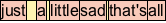
\includegraphics[height=0.5cm]{img/s3_16_0113.png} \\
\end{tabular}
%\hfill
\\
\begin{tabular}{c}
Prosodic translation \\
Es un poco [P] triste, eso es todo. \\
\end{tabular}
\caption{Prosodic translation of segment s3\_16\_0113 from the Heroes corpus.}
\label{transprose:figure:q3:goodone1}
\end{figure}

\begin{figure}[h!]
\centering
\begin{tabular}{c}
Input segment \\
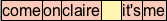
\includegraphics[height=0.5cm]{img/s3_1_0001.png} \\
\end{tabular}
%\hfill
\\
\begin{tabular}{c}
Prosodic translation \\
venga, claire. [P] soy yo. \\
\end{tabular}
\caption{Prosodic translation of segment s3\_1\_0001 from the Heroes corpus.}
\label{transprose:figure:q3:goodone2}
\end{figure}
%TODO: \mireia{Figures are a little bit confusing, in the same way there where in chapter 4. I don't come up with a clearer visualisation, but maybe putting input segment and prosodic translation in a left column and prosograph segment and translation on the right} 

Examples like these show that the model does learn to predict pauses in translations to some extend. However, the size of the training set shows to be too small to obtain useful generalizations for this problem. 

\subsubsection{Perception tests with text-to-speech synthesis}
A perception test was prepared to test to what extend the pausing cues outputted by the prosodic translation actually help. This test involved participants listening to a batch of original segments from the Heroes corpus and then listening to two types of synthesized translations (dubbings): (1) synthesis of the ``classical'' text translation output, and (2) synthesis of the prosodic translation together with the prosodic cues. Two comparisons were made for each sample pair: 

\begin{enumerate}
    \item Which one of the Spanish dubbings is a better translation of the original English segment? 
    \item Which one of the dubbings better reflects the prosody of the original speech?
\end{enumerate}


\textbf{Selecting the samples} It was challenging to select the samples to be used in such a test for two reasons: firstly, the quality of translations was, in general, considerably low. If a fair comparison has to be made, both outputs of the text translation model and the prosodic translation model had to be with an acceptable quality. This was assured by manually picking samples from the testing set which had acceptable translations for both models. Secondly, if a prosodic comparison was to be made, there had to be a prosodic cue output on the prosodic model. As reported earlier, only one quarter of the prosodic translations of the testing set actually had a pausing output given that there was a pausing in the source English sentence. 15 sentences were selected respecting these requirements. 

\textbf{Synthesizing the translations} IBM Watson TTS \footnote{\url{https://www.ibm.com/watson/services/text-to-speech/}} was used to obtain synthesized versions of the translations. This service is provided free of charge and offers inputting of prosodic conditioning with SSML tags \citep{ssml}. In this case, it was only needed to add breaks after the words with a pause after on the prosodic translations. Lengths for the breaks were selected regarding the average lengths of breaks in the Spanish segments. 

%TODO: \mireia{I would insert a table with the percentages to improve readability}

\textbf{Results} 32 people participated in the test. The results of the perception test show that in 76.5\% of the cases the translation made by the prosodic model was preferred. However, in prosodic assessment, synthesized samples with the prosodic cues were preferred in only 27\% of the cases. In 32.4\% of the cases, participants stated that they heard no difference between the synthesized samples in terms of prosody. The majority 40.6\% preferred synthesized version of the text translation. 

The lack of agreement on synthesized samples can be explained by two reasons: firstly, both synthesized samples were greatly far from the original segments from the series. Many participants found the dubbings highly ``robotic'' after hearing an original actors version from the TV series. Second reason is that in many samples the added pauses contributed even more to the unnaturalness of the synthesized samples. This shows that the pauses cannot be taken in isolation from other prosodic cues. Appearance and duration of the pauses are directly affected by the speech rate. In turn, a pause between two words affects the general intonation of the sentence. If the pause for example is placed for emphasis, the emphasized word should be marked with a high pitch or intensity as well. Placement of a pause without taking account the general prosodic structure does not contribute in terms of expressivity and even might harm it in terms of naturalness. 

%It might be good to list the results here and argue that the outputs are highly related with punctuation. 

\section{Conclusion}

%Motivation, and what was done in a glance
In this chapter, I have discussed about the reasons and ways to include prosodic features in a spoken language translation pipeline. I formed my motivation on the use-case of automatic translation and dubbing of media material such as movies or TV shows. A prosodically enhanced neural machine translation system was proposed. Experiments were performed using a parallel corpus compiled from the original and dubbed spoken segments from movie domain.

%Study
The empirical study performed on the segments of the Heroes corpus indicate that pauses have an effect both on the translation and dubbings made by professionals. In majority of cases both original and dubbed speech segments agree on containing an inter-lexical pause. I used these findings to argue that if an automated system was to be built to translate and dub spoken segments in a TV show, it has to heed certain prosodic characteristics of the actors' speeches just as dubbing artists do. I further demonstrated how the classic speech-to-speech translation pipeline would fail to do a proper translation when prosody of the source sentence is ignored.

%Model and training
Motivated by the shortcomings of this classic translation pipeline, a novel framework has been introduced that takes prosodic features into account and outputs prosodic cues for the synthesis of the translated segments. This framework, which I call \textit{TransProse}, is designed to take speech transcriptions together with their word-level prosodic features and output translations with word-level prosodic cues. Joint prosodic-textual translation models were trained in two stages, where in first stage translation of word tokens is learned from a large corpus from movie domain and later transfer of prosodic features are learned on a second stage from a corpus annotated with prosodic-acoustic features.

%Questions and experiments
My experiments involving the incorporation of prosody to the movie-domain translation pipeline were built around these three questions: (1) How does prosodic punctuation restoration affect translation?, (2) Does pause encoding improve translation? and (3) Can pauses be translated jointly with lexical information? Through these three questions I have employed prosody into the TransProse translation pipeline in three steps. In the first step prosody is incorporated on the standard text-to-text translation setting by punctuating the source sentences using prosodic cues. In the second step, inter-lexical pausings as the sole prosodic features is introduced on the encoder side to improve the translations. And finally on the third step, I introduced both prosodic input and output where the output tokens were accompanied with flags that signal if a pause should be placed after a lexical element or not.  

%Good Results on prosodic encoding (1) punctuation
As my initial study suggested, improvements over the translation quality were achieved with incorporation of prosody into the input side of the translation framework. Related to my first question, I reported an improvement over usage of prosodic features in a preliminary punctuation restoration step. This was demonstrated with automatic punctuation recovery in the input phrases using first solely lexical features and then lexical-prosodic features. It showed that punctuation recovery on input phrases improves a lot the translation quality in movie domain. Lexical-based punctuation recovery recorded an improvement in terms of 4.77\% BLEU over the unpunctuated input. However, a translation model that was trained to recover punctuation on target phrases performed better (5.27\% BLEU increase) without an additional punctuation recovery process. Finally, the lexical-prosodic punctuation recovery was employed on the input sentences. This setting worked the best in terms of translation quality given unpunctuated input sentences with a BLEU improvement of 5.91\% compared to unpunctuated input. The experiment showed that a prosodic punctuation recovery step before translation serves best for overall translation quality. 

%(2) prosodic encoding
For answering my second question, I have incorporated inter-lexical pauses to the translation pipeline and assessed its effect on the translation quality. Comparing with standard text translation an improvement of 1.31\% BLEU was achieved with incorporation of pause feature on the input side. To demonstrate this increase in a setting closer to a real speech-to-text translation setting, punctuation marks in the input phrases were removed (which would be missing in ASR output) and recovered again using the prosodic punctuation models and a similar improvement has been recorded (1.07\%). The results clearly show the usefulness of including prosodic features in a spoken translation pipeline. This proved my hypothesis that pausing could act as a cue in machine translation just like punctuation, given their co-presence and abundance especially in movie domain. Incorporation of more prosodic features should be considered in future research. 

%(3) cues for synthesis
The final experiment presented in this section delved into the task of spoken output with the motivation of further work in a full speech-to-speech translation pipeline. I have demonstrated that through the proposed framework it is possible to obtain some meaningful output to be used as cues in a text-to-speech system. However, low performance on text translation certainly hindered the process of evaluation since it was difficult to assess the correct placement of pauses on a different translation than the reference translations. To account for this, a smaller and cleaner test set was prepared. Manual inspection on output in this set also failed in demonstrating a successful transfer of pausing within a joint prosodic-lexical translation architecture. This can partially be explained by the non-standard transfer of pauses in the data, such as silent pauses being dubbed as filled pauses etc. Also, it could be a problem in the architecture. Pause encoding has to pass through many layers in the architecture until the pause flag output layer, which is connected through the more strongly trained lexical path. It is possible that pause information gets lost in the way with this setup. Techniques like skip-encoding \citep{Quoc2017} of prosodic features can be a remedy for this. 

%perception tests
Further perception tests were performed on a selected meaningful set of sample outputs with pause information to see the feasibility in using this type of output for synthesis. A state-of-the-art TTS system was employed to synthesize these translations with the pause intervals coded as breaks. Participants were asked to compare them with the synthesized samples of the regular text translations. In average, prosodic translations were preferred in terms of translation but not in terms of closeness to the original samples from the series. The conclusion from this experiment was that single prosodic features cannot be considered as isolated from other features. In order to achieve a complete transfer of suprasegmental prosodic features, many aspects should be considered as a whole such as transfer of spectral characteristics, speech rate, intonation, etc. in a TTS system. 

%conclusion on future of movie domain slmt 
All in all, the proposed methodology paves the way for research for inclusion prosody in both neural speech-to-text and speech-to-speech translation pipelines. Even with a simple model and a limited sized audio data it is possible to achieve improvements on spoken language translation in movie domain through incorporation of prosody. 

Next chapter, I will conclude the thesis with final remarks and possible future work. 